\documentclass[10pt]{article}

\usepackage{spheric}
%%%TITLE
\title{A SPH model for the root system of plants}
\date{}

%%AFFILIATIONS
\author[1]{Matthias MIMAULT$^\dagger$}
\author[1]{Lionel DUPUY}
\affil[1]{James Hutton Institute, UK}
\author[2]{Mariya PTASHNYK}
\affil[2]{University of Dundee, UK}

\affil[$\relax$]{\email{\dagger}{matthias.mimault@hutton.ac.uk}}


%%DOCUMENT
\begin{document}

\maketitle

%\SelectedTopics{Biomechanics, Multiple Continua and Multi-Phase Flows and Solids and structure}

%%PLEASE PUT YOUR ABSTRACT HERE
\begin{abstract}
Feeding more than 9 billion people will require a more reasonable use of water fertilizers and a good understanding of the mechanics of plant growth in soil. Unfortunately, experimenting biology and physics of growth in soil is difficult because live in situ observation of roots is extremely limited. Methods for measurement of roots are often destructive and time consuming, and knowledge of the process limiting growth in soil is lacking \cite{smit2013root}. Mathematical modelling proved a useful approach to bridge this knowledge gap, but current models fail to incorporate the role of cellular processes at the organ level \cite{smith2006plausible}. The objective of this work is to develop a cellular model for root growth solved at the macroscopic level using the Smoothed Particle Hydrodynamics method (SPH). 

Our SPH model is based on the structural similarity of the root cells with the SPH particles, to solve macroscopic physical processes while modelling autonomous biological process at the level of the cell. We identify the cellular elongation and division as principal drivers of the growth. As the deformation of tissues occurring during growth is conducted by the Turgor pressure, we define our growth model in the framework of the poroelastic theory. Here the pore pressure is a consequence of cellular activity and subsequent chemical gradient within cells. Along with it, we include cell division with particle splitting. This division is controlled biologically, according to the chemical level distribution and located at the tip of the root, called the ``meristem''. Once divided, the cells are moving away from the meristem and growth therefore is dominated by elongation. We discuss here the effect of those mechanisms in a poroelastic model and illustrate this approach with study cases. We also show how such models integrate within the SENSOIL project that combines innovative imaging systems and experiments.


\begin{figure}[!htb]
\centering
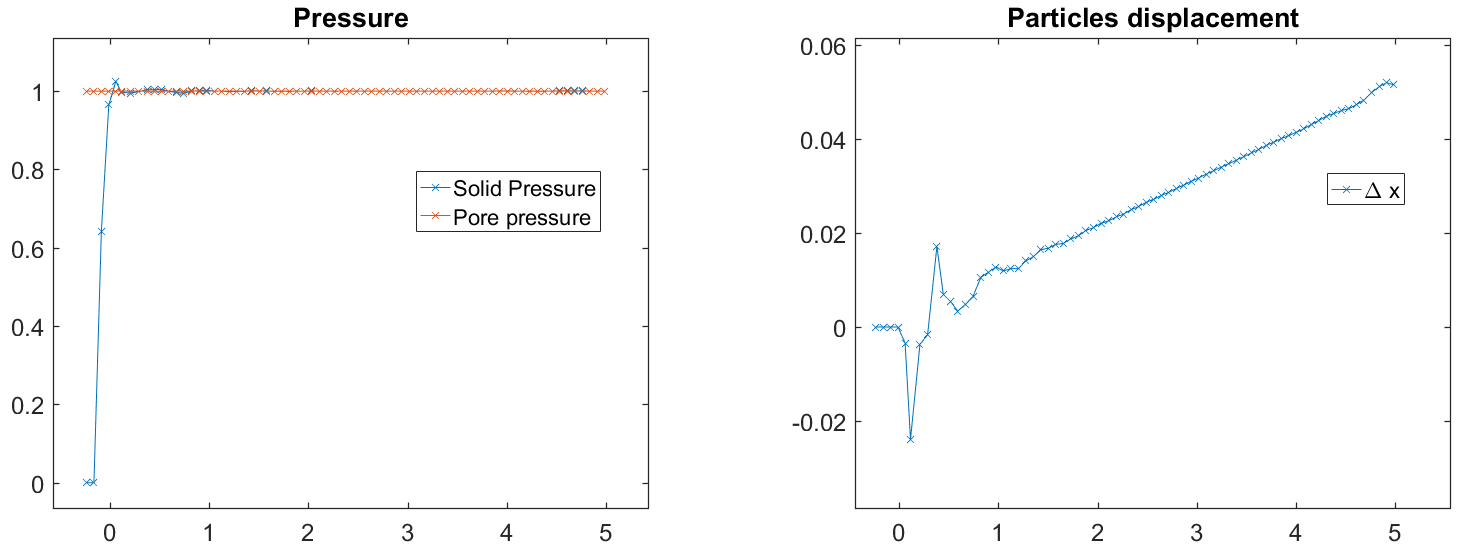
\includegraphics[width=0.95\textwidth]{3-11.png}
\caption{Pressure and displacement of particles in a 1D sample at equilibrium with imposition of a constant pore pressure and fixed left boundary. 200 particles for a cell size of 2.5 $\mu\mathrm{m}$. Values in mm and kPa.}\label{fig:3}
\end{figure}

\end{abstract}


%%THE END OF ABSTRACT

\addbib

\end{document}
